\chapter{Reproduction in Plants}

\section{Get rolling}

\textbf{Vidya is going to have delicious \textit{jeera} (cumin) rice and \textit{rajma} (kidney beans) for lunch.}
\par
Do you know what cumin, rice and kidney beans have in common? They all are \textbf{seeds.}
\par
We eat the seeds of some plants as food. Name some more seeds that you eat.

\section{\textcolor{red}{What to Know}}
Structure, germination and dispersal of seeds, and growth of plants from parts like roots, stems and leaves
\section{\textbf{Learning Objectives}}

\begin{itemize}
    \item to examine the structure of a seed
    \item to study germination of a seed
    \item to describe the different modes of seed dispersal
    \item to identify parts other than seeds that can be used to grow new plants
    \item to describe the types of crops
\end{itemize}
\section{\textcolor{red}{Seeds}} 
A lot of green plants are flowering plants. Flowers turn into fruits. Fruits contain seeds. Underfavorable conditions, seed grow into new plants.
\subsection{\textcolor{orange}{Structure of a Seed}}
Let us learn about the structure of a seed with the help of a activicty.\\
\par
The internal structure of a seed is shown in the picture.\\
\par
A seed is covered by a \textbf{seed coat} which protects it. Inside the seed coat, the seed has fleshy seed leaves known as \textbf{cotyledons.} Cotyledons store food to provide nutrition to the growing embryo.\\
\par
An \textbf{embryo} is a baby plant present inside a seed.\\ 
\par
Some seeds have two cotyledons and some seeds have only one. Seeds with two cotyledons are called \textbf{dicot seeds.} Examples include peas, beans and pulses. Seed with one cotyledon are called \textbf{monocot seeds.} Examples include maize, rice and wheat.
\section{\textcolor{red}{Germination of a Seed}}
An adequate supply of air, water and warmth helps seeds to \textbf{sprout}. When a seed sprouts, is embryo develops into a new plant. The process by which a seed develops into a new plant or a seedling is called \textbf{germination.}
\begin{figure}
    \centering
    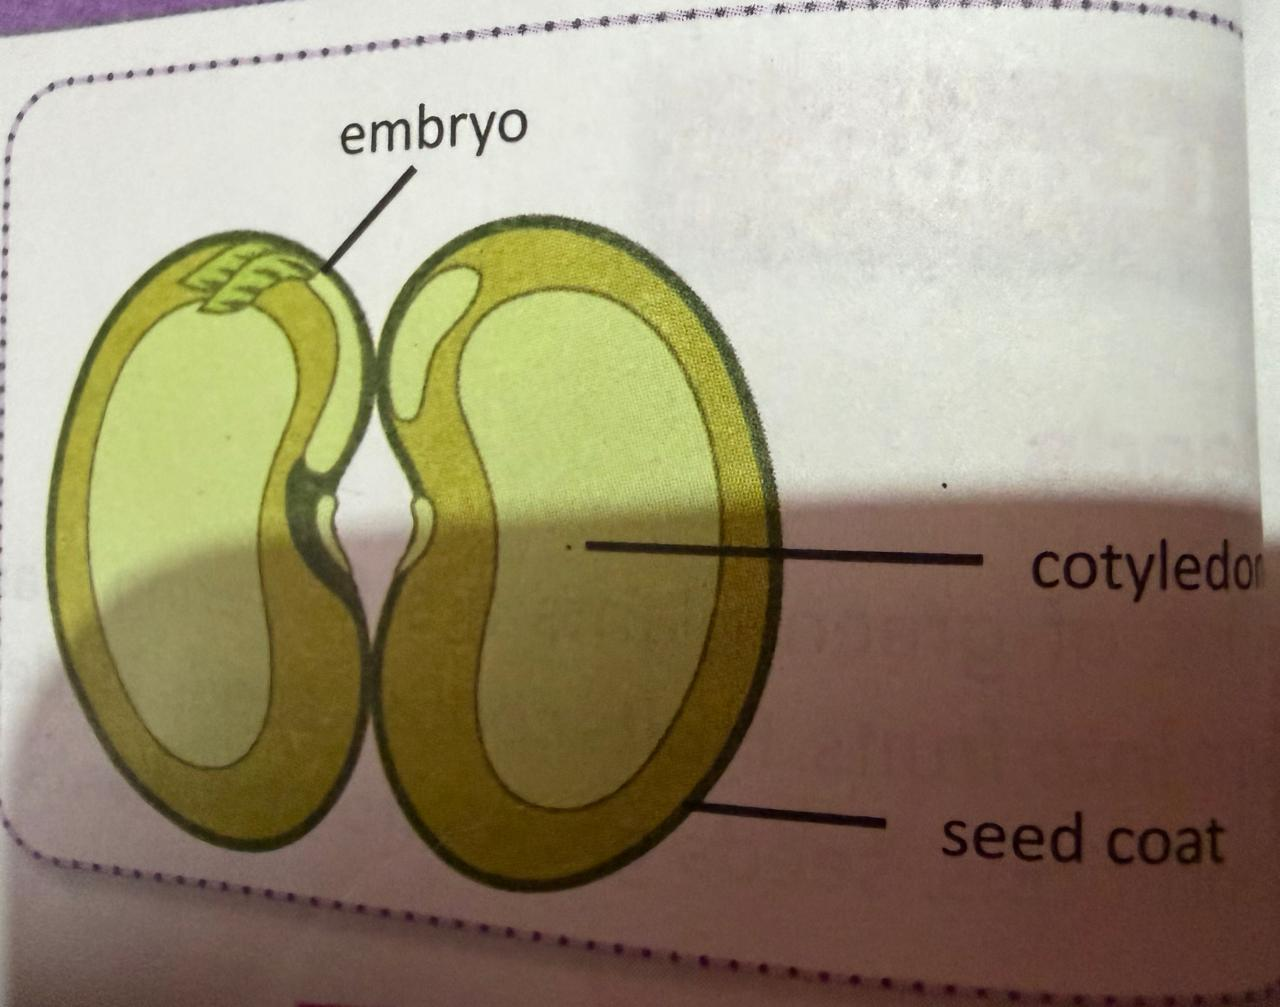
\includegraphics[width=0.5\linewidth]{../image/Structure_of_a_seed.jpeg}
    \caption{Caption}
    \label{fig:seed}
\end{figure}
\subsection{\textcolor{orange}{Stages of Germnation of a Seed}} 
Stage 1: When a seed gets water, it swells and becomes soft.\\
Stage 2: A tiny root called the \textbf{radicle} starts to grow out of the seed. It goes down into soil, looking for water and nutriients.\\
Stage 3: While the radicle is busy going into soil, a little shoot called the \textbf{plumule} grows upwards. It pushes its way up through the soil, reaching for sunlight. The plumute becomes the stem (shoot) and gives rise to the leaves of the plant.\\
Stage 4: As the shoot and root keep growing, the seed becomes a small plant called a \textbf{seedling.}\\
Stage 5: The seedling grows using the food stored in the cotyledon or cotyledons. It then grows leaves to make food.
\begin{figure}
    \centering
    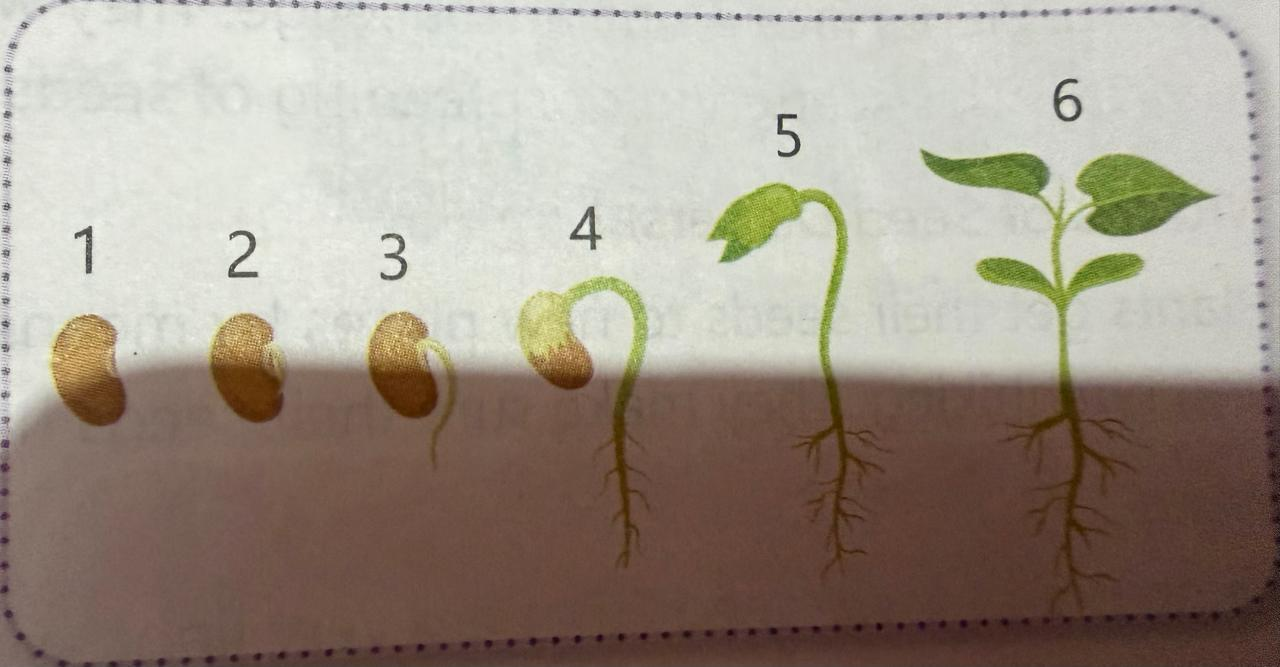
\includegraphics[width=0.5\linewidth]{../image/Germination_of_a_seed.jpeg}
    \caption{Caption}
    \label{fig:germination}
\end{figure}
\section{\textcolor{red}{Dispersal of seeds}} 
Plants stay at one place, but their seeds travel. To ensure that seeds don't just drop nearby, plants have different ways of sending then away. Why?\\
\par
Think about being stuck in a crowded place with little food and water. It would be tough to survive. Plants face a similar challenge. They want their seeds to go far and find new places to grow. This scattering or spreading of seeds is called a \textbf{seed dispersal.}
\subsection{\textcolor{orange}{Modes of Seed dispersal}}
Plants get their seeds to new places by means of wind, animals, water, seedpod explosions and hitchhiking. They make sure their seeds have the best chance to grow into new plants.
\subsection{\textbf{Wind}}
Some plants have seeds that are very light, with tiny parachutes, wings, hair or feathers. When wind blows, these seeds get carried away, floating through the air. Eventually, they land in a new place, where they can grow new plants.
\begin{figure}
    \centering
    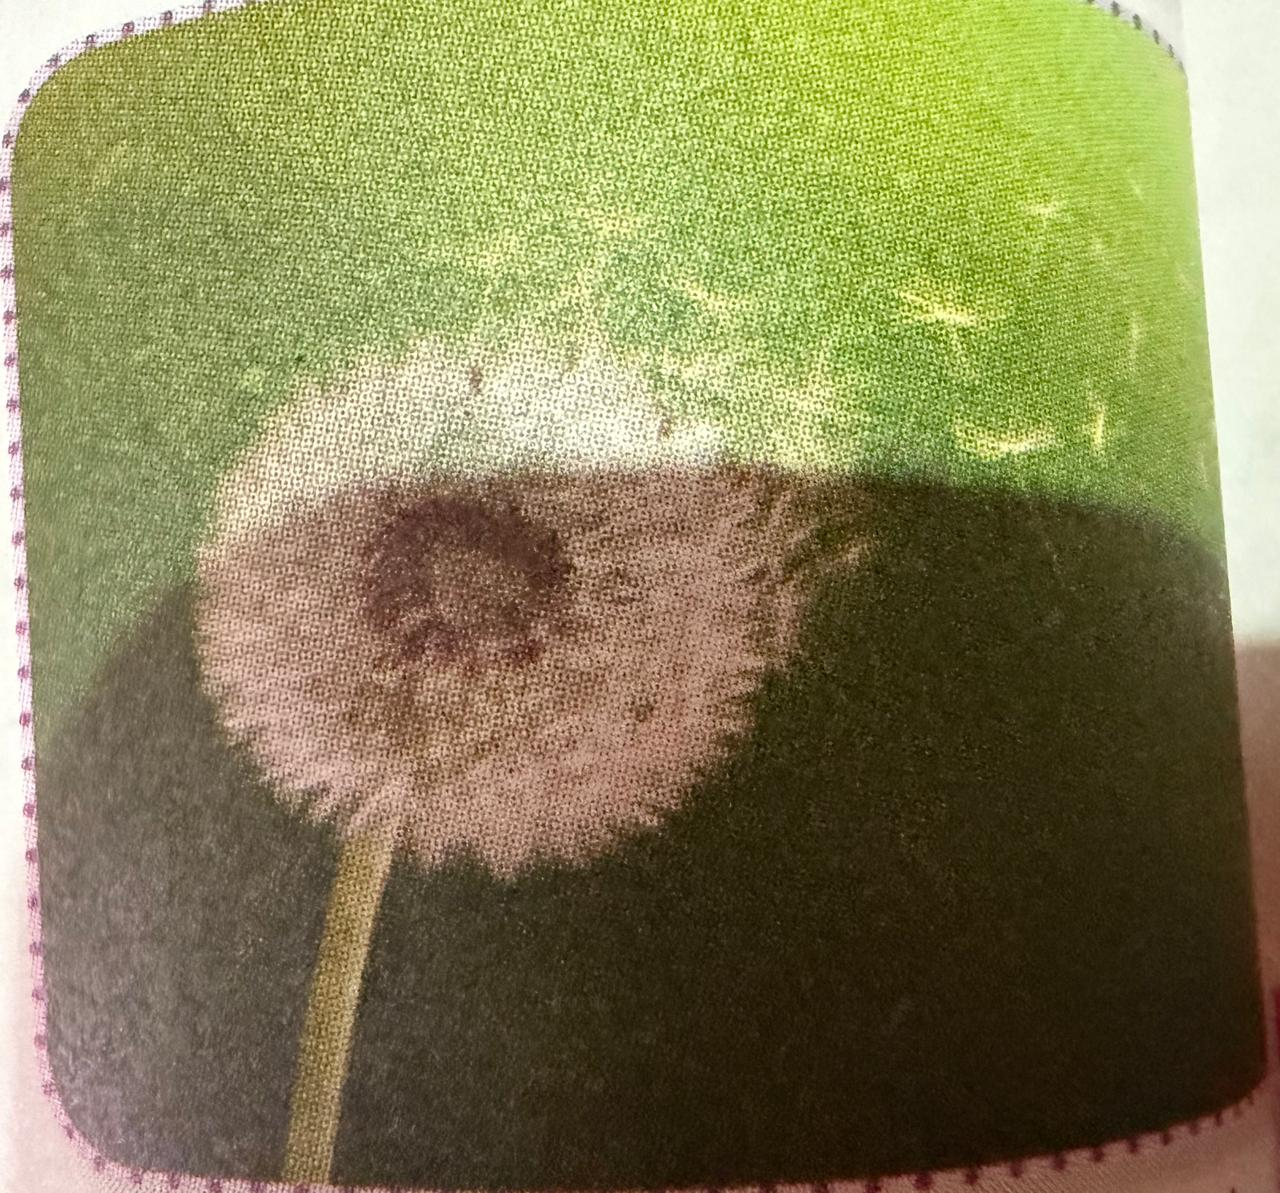
\includegraphics[width=0.5\linewidth]{../image/dandelion_seed.jpeg}
    \caption{Caption}
    \label{fig:dandelion}
\end{figure}
\subsection{\textbf{Animals}}
Animals can also help plants in seed dispersal. Some plants have seeds that are enclosed in fruits and animals. The animals eat the fruits or seeds and they drop the seeds or leave them behind in their droppings as they travel. 
\begin{figure}
    \centering
    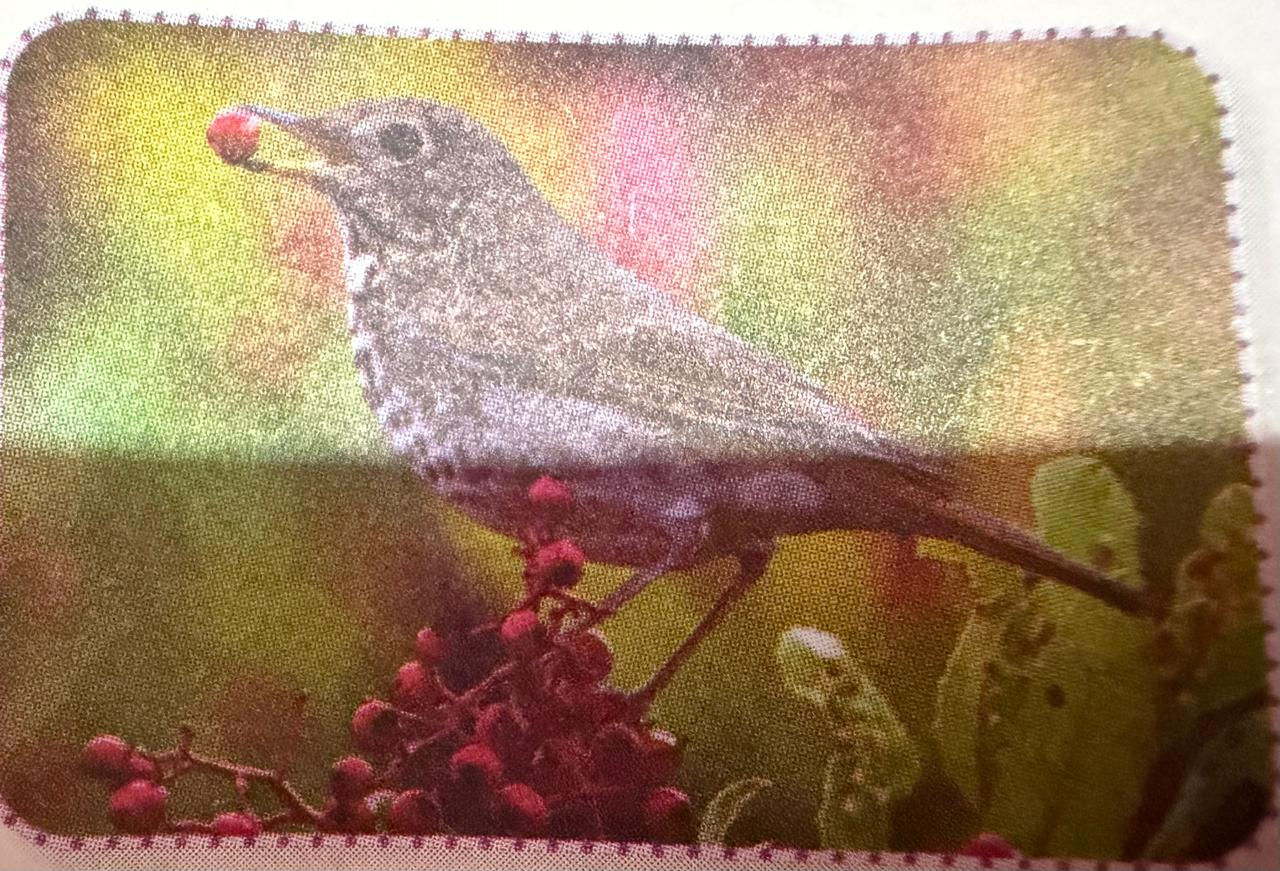
\includegraphics[width=0.5\linewidth]{../image/birds_eating_berries.jpeg}
    \caption{Caption}
    \label{fig:bird}
\end{figure}
\subsection{\textbf{Water}}
Some plants live in or near water bodies like seas, rivers and lakes. They have seeds that can float in water. When the seeds fell into water, they flow with the waves until they reach the shore. There they start growing into new plants.
\begin{figure}
    \centering
    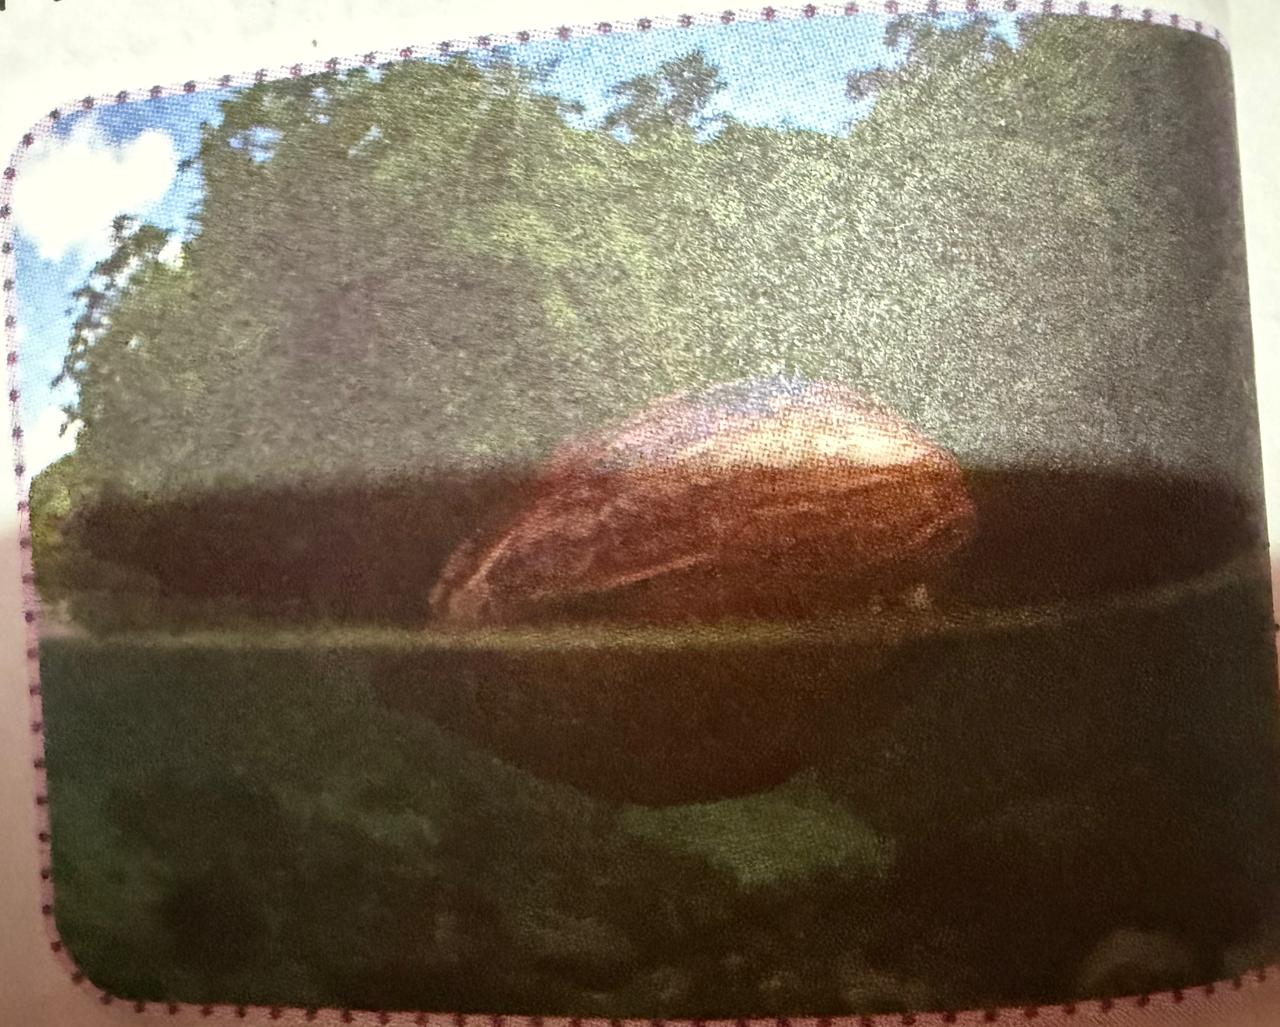
\includegraphics[width=0.5\linewidth]{../image/cocunut_seed.jpeg}
    \caption{Caption}
    \label{fig:coconut}
\end{figure}
\subsection{\textbf{Seedpod Explosions}}
Have you ever seen a plant that suddenly brust its seedpods open and shoot out the seeds? It is like a tiny explosion. These plants have seeds that are contained in seedpods. When the pods dry out, they split open, scattering the seed all directions. This helps seeds spread out and find new places to grow. Pea and ladyfinger plants explode their seedpods.
\begin{figure}
    \centering
    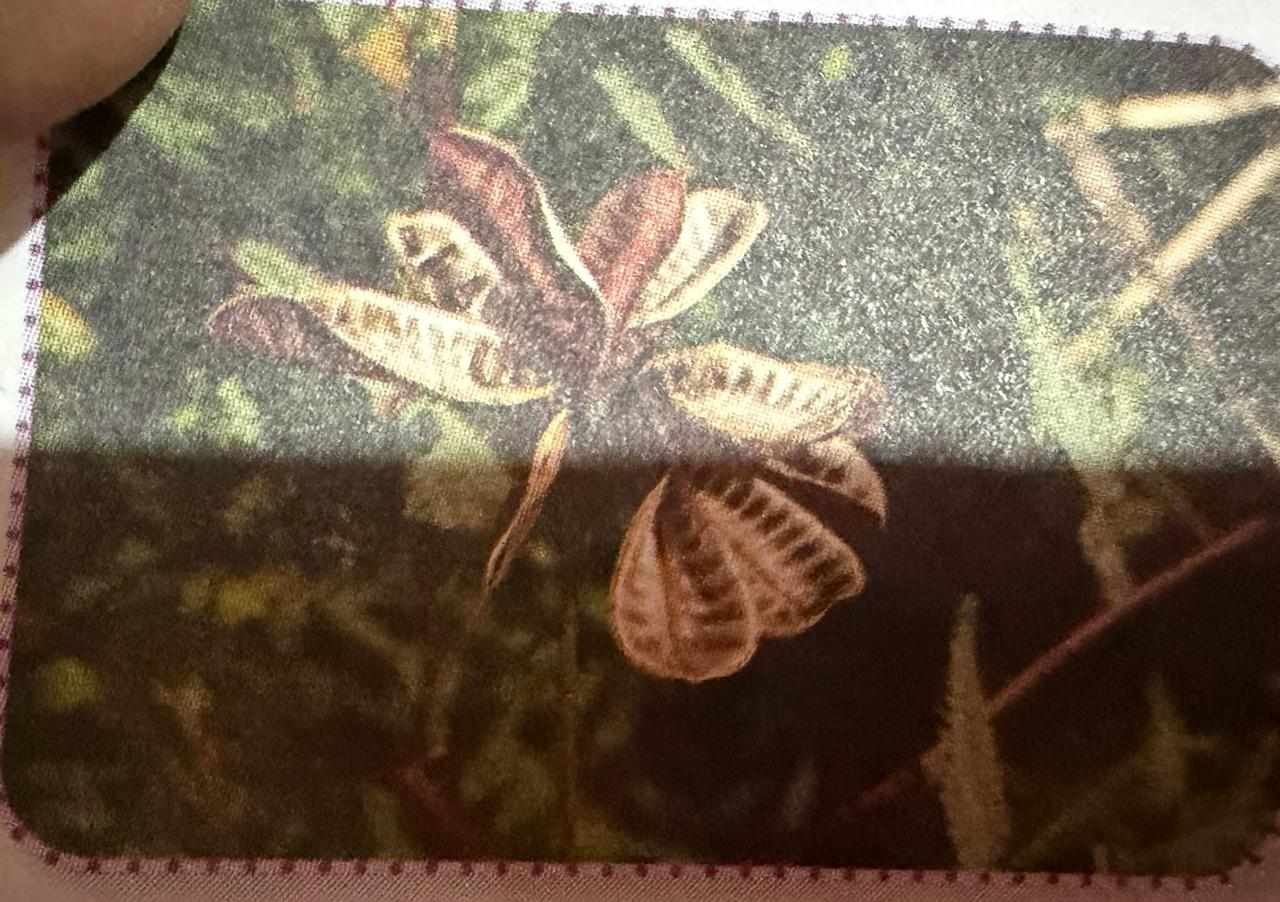
\includegraphics[width=0.5\linewidth]{../image/seedpod_explosion.jpeg}
    \caption{Caption}
    \label{fig:seed-pod}
\end{figure}
\subsection{\textbf{Stick and} \textcolor{red}{Hitchhike}}
Some plants have seeds with special hooks or spines that can stick to the fur or feathers of animals. As the animals move around, the seeds take a ride with them. When the animals brush against other plants or shake themselves, the seeds get detached and fall to the ground, ready to grow.\\
\par
\textcolor{red}{I wonder} if humans help in seed dispersal!
\section{\textcolor{red}{Reproduction of Plants Without Seeds}}
\textbf{Vegetative propagation} is a method of growing new plants without using seeds. Instead of starting from a seed, vegetative propagation involves using part of an existing plants, such as its roots, stems or leaves to reproduce a new plant.
\begin{figure}
    \centering
    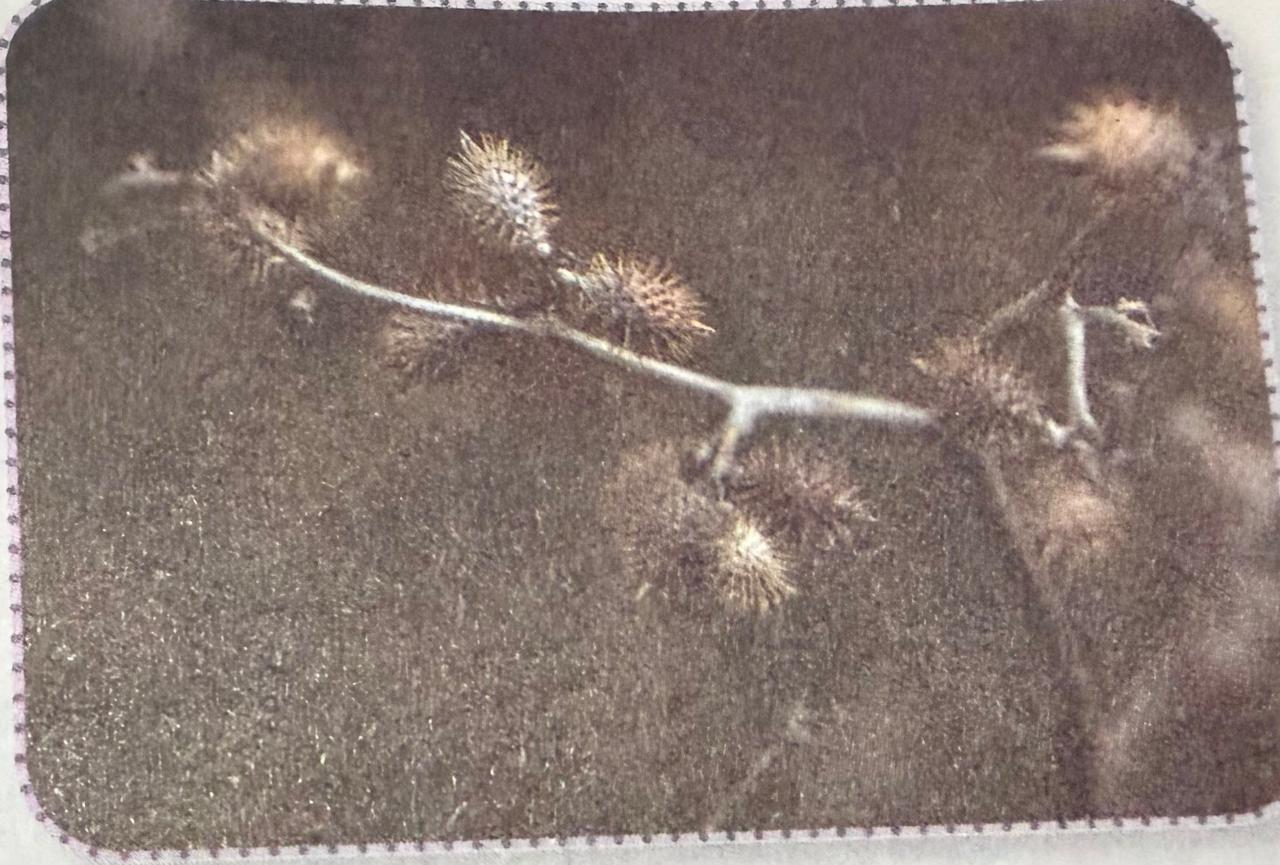
\includegraphics[width=0.5\linewidth]{../image/Stick_and_hitchike.jpeg}
    \caption{Caption}
    \label{fig:stick}
\end{figure}
\subsection{\textcolor{orange}{Growing Plants from Roots}}
Plants such as carrots, radishes, turnips and sweet potatoes have swollen roots. The roots are swollen because they store food. When these roots are put in the soil, they give rise to new plants.
\subsection{\textcolor{orange}{Growing Plants from Stems}}
The part of the stem is cut and planted in soil. It develops roots after some time and finally grows into a whole new plant. This method is called \textbf{stem cutting.}
\par
\begin{figure}
    \centering
    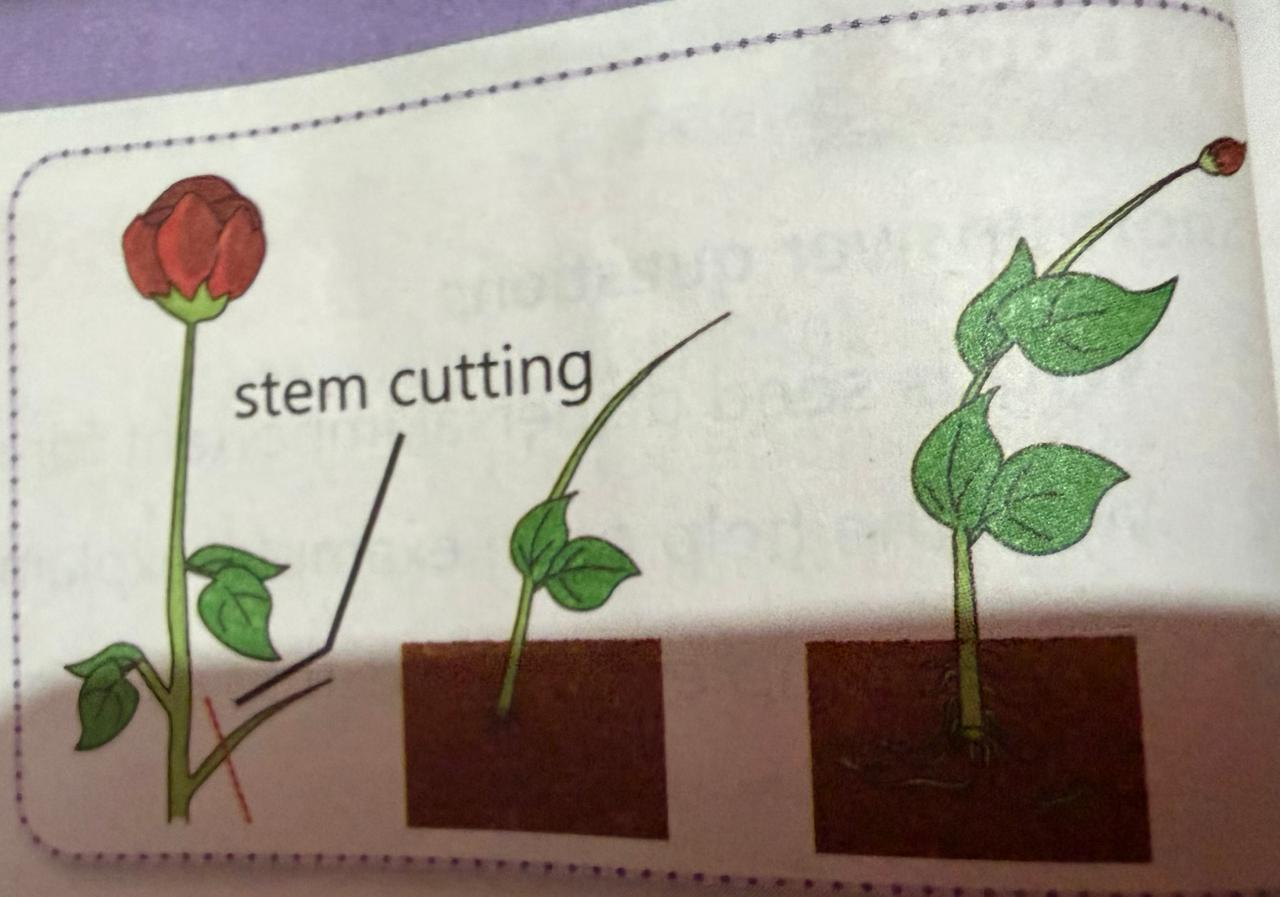
\includegraphics[width=0.5\linewidth]{../image/stem_cutting.jpeg}
    \caption{Caption}
    \label{fig:stem-cutting}
\end{figure}
Plants like mint, rose, hibiscus and money plant reproduce by stem cutting.

\subsection{\textcolor{orange}{Growing Plants from Leaves}}
Plants such as \textit{Bryophyllum} grow from leaves. These leaves have small buds on their margins. The buds separate from the leaves, fall to the ground and give rise to new plants.
\par

\begin{figure}[h]
    \centering
    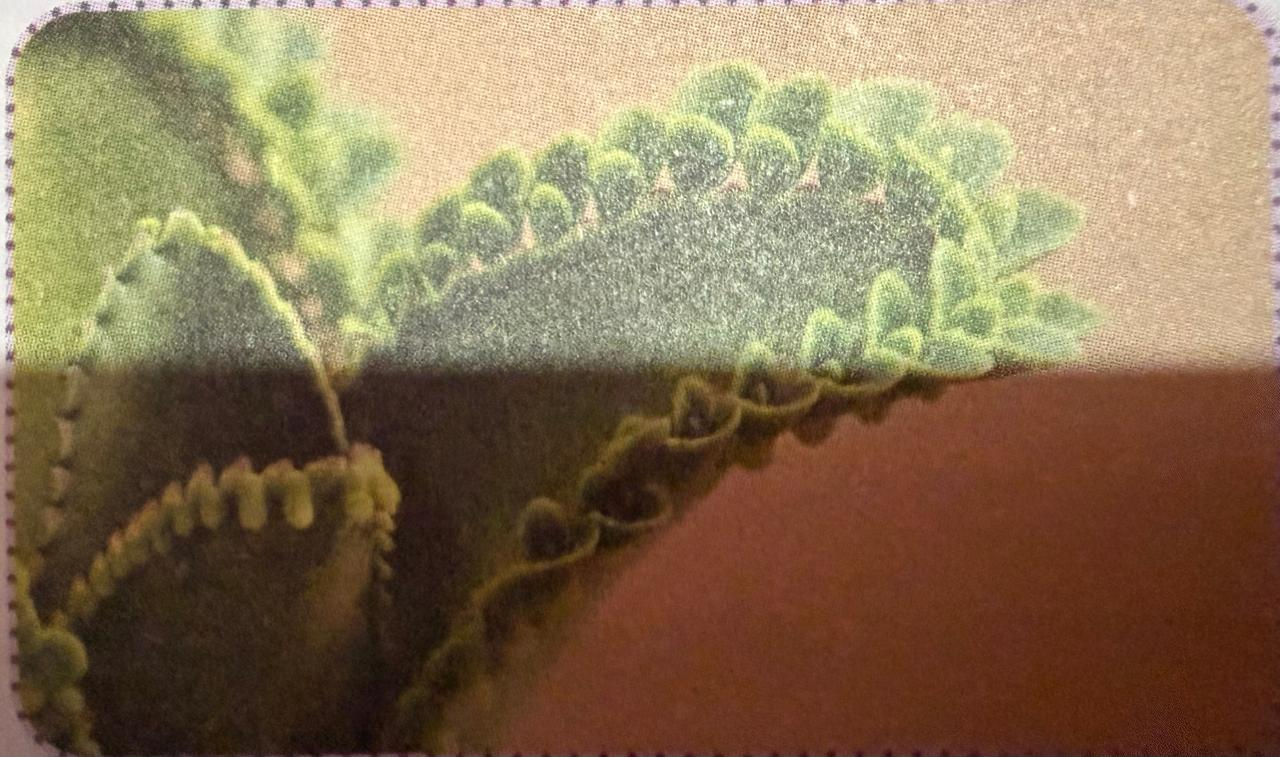
\includegraphics[width=0.5\linewidth]{../image/bryophyllum_leaf.jpeg}
    \caption{Leaf}
    \label{fig:leaf}
\end{figure}

\section{\textcolor{red}{Crops and their Types}}

\textbf{Crops} are plants that people grow on farms on a large scale. They are plants that are grown for various purposes. Some crops are grown for the food they provide such as fruits, vegetables, grains (like rice or wheat) and nuts.

\par
Some crops are grown for other purposes. For example, cotton is grown to make clothes and fabrics.\\
\par
The science or particle of growing crops on large scale is called \textbf{agriculture.}\\
\par
In India, depending on the time of the year of the season in which they are grown, crops are divided into two types - kharif and rabi crops.
\subsection{\textcolor{orange}{Kharif Crops}}
\textbf{Kharif crops} are sown in during the rainy season, which typically begins around June and lasts until September. These crops are depend on the monsoon rains. Some examples of kharif crops include rice, maize, millets, groundnuts, cotton and sugarcane.
\begin{figure}
    \centering
    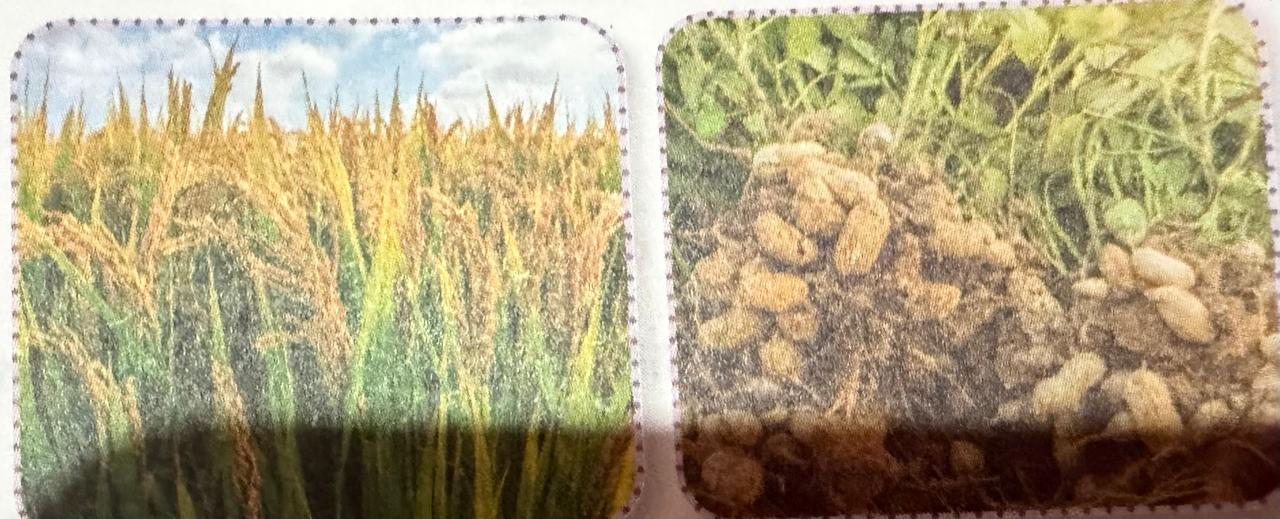
\includegraphics[width=0.5\linewidth]{../image/Kharif_crops.jpeg}
    \caption{Caption}
    \label{fig:kharif}
\end{figure}
\subsection{\textcolor{orange}{Rabi Crops}}
\textbf{Rabi crops} are sown in winter, usually from October to December. These crops rely on winter rainfall. Some examples of rabi crops include wheat, barley, mustard and potatoes.
\begin{figure}
    \centering
    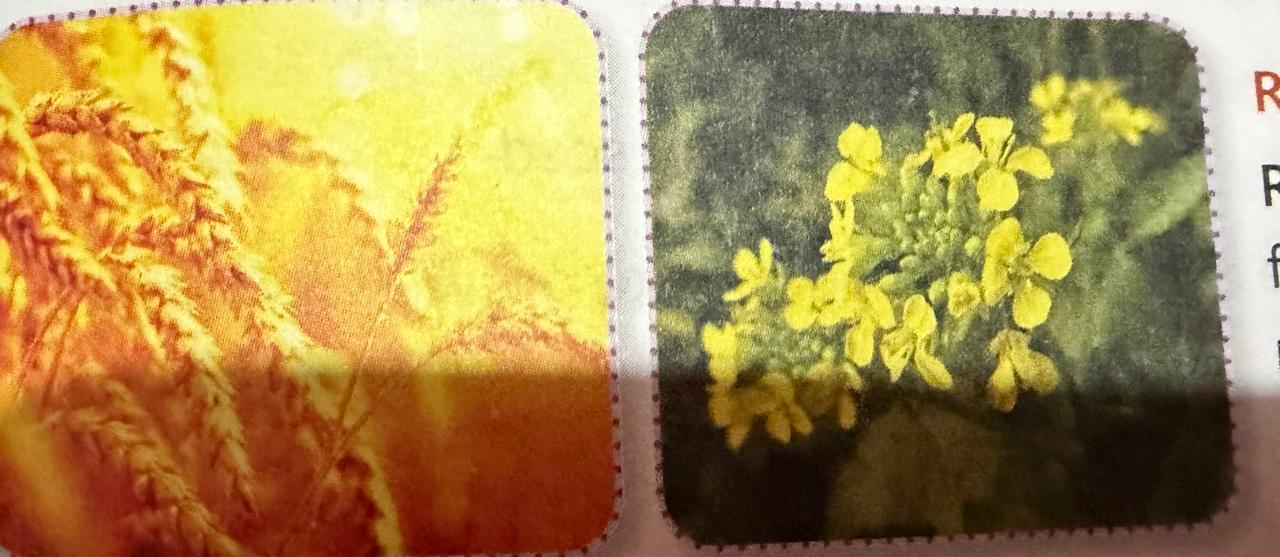
\includegraphics[width=0.5\linewidth]{../image/rabi_crops.jpeg}
    \caption{Caption}
    \label{fig:rabi}
\end{figure}
\begin{itemize}
    \item Plants can grown from seeds and some othe parts such as roots, stems and leaves.\\
    \item A seed consists of a seed coat, a cotyledons and an embryo.\\
    \item Whenever seeds get favourable conditions (i.e., proper air supply, warmth and water), they sprout and this process is called \textbf{germination.}\\
    \item Plants ensure that seeds are scattered far away from them to get proper space, sunlight, water and nutrients. This process of scattering seeds is called \textbf{seed dispersal.}\\
    \item Wind, water or animals help in seed dispersal of many plants.\\
    \item \textbf{Vegetative propagation} is a method of plant reproduction without seeds.\\
    \item \textbf{Crops} are plants people grow on farms on a large scale. Two types of crops are grown in India - kharif crops (monsoon crops) and rabi crops (winter crops).\\
\end{itemize}